% https://es.overleaf.com/latex/templates/project-report/jpzczmpsdzwm

%%% Preamble
\documentclass[paper=leter, fontsize=11pt]{scrartcl}
\usepackage[utf8]{inputenc}
\usepackage[spanish,mexico]{babel}
\usepackage[T1]{fontenc}    % use 8-bit T1 fonts
\usepackage{lmodern}
\usepackage{hyperref}       % hyperlinks
\usepackage{lipsum}
\usepackage[square,numbers]{natbib}

\usepackage[protrusion=true,expansion=true]{microtype}	
\usepackage{amsmath,amsfonts,amsthm} % Math packages
\usepackage[pdftex]{graphicx}
\usepackage{url}
 
\usepackage{booktabs}
\usepackage[table,xcdraw]{xcolor}

\usepackage{tikz}
\usetikzlibrary{positioning,matrix, arrows.meta}

\usepackage{caption} 
\usepackage{subcaption}


\usepackage{listings}
\lstdefinestyle{mystyle}{ 
    basicstyle=\ttfamily\footnotesize,
    breakatwhitespace=false,         
    breaklines=true,                 
    captionpos=b,                    
    keepspaces=true,                 
    numbers=left,                    
    numbersep=5pt,                  
    showspaces=false,                
    showstringspaces=false,
    showtabs=false,                  
    tabsize=4
}

\lstset{style=mystyle}
\renewcommand{\lstlistingname}{Código}


\selectlanguage{spanish}
\usepackage[spanish,onelanguage,ruled]{algorithm2e}


%%% Custom sectioning
\usepackage{sectsty}
\allsectionsfont{\centering \normalfont\scshape}


%%% Custom headers/footers (fancyhdr package)
\usepackage{fancyhdr}
\pagestyle{fancyplain}
\fancyhead{}											% No page header
\fancyfoot[L]{}											% Empty 
\fancyfoot[C]{}											% Empty
\fancyfoot[R]{\thepage}									% Pagenumbering
\renewcommand{\headrulewidth}{0pt}			% Remove header underlines
\renewcommand{\footrulewidth}{0pt}				% Remove footer underlines
\setlength{\headheight}{13.6pt}


%%% Equation and float numbering
\numberwithin{equation}{section}		% Equationnumbering: section.eq#
\numberwithin{figure}{section}			% Figurenumbering: section.fig#
\numberwithin{table}{section}				% Tablenumbering: section.tab#


%%% Maketitle metadata
\newcommand{\horrule}[1]{\rule{\linewidth}{#1}} 	% Horizontal rule

%%% https://tex.stackexchange.com/a/118217
\usepackage{mathtools}
\DeclarePairedDelimiter\ceil{\lceil}{\rceil}
\DeclarePairedDelimiter\floor{\lfloor}{\rfloor}

\usepackage{amsmath}

\usepackage{tikz}

\title{
		%\vspace{-1in} 	
		\usefont{OT1}{bch}{b}{n}
		\normalfont \normalsize \textsc{Posgrado de Ingeniería de Sistemas} \\ [25pt]
		\horrule{0.5pt} \\[0.4cm]
		\huge Generadores pseudoaleatorios \\
		\horrule{2pt} \\[0.5cm]
}
\author{
		\normalfont 								\normalsize
        Alberto Benavides\\[-3pt]		\normalsize
        \today
}
\date{}


%%% Begin document
\begin{document}
\maketitle

\section{Introducción}

Una máquina es determinista y, por sí misma, no puede generar números aleatorios. Existen estrategias para conseguirlo, como las utilizadas por \citet{random} que lo hace a partir de ruido ambiental. De todas formas, existen algoritmos que se utilizan para generar números pseudoaleatorios. Entre ellos figuran un generador definido por el \textit{método de Box--Muller} o el llamado \textit{generador lineal congruencial}.

\section{Método Box--Muller}
El método de Box--Muller parte de dos números pseudoaleatorios $u_1$ y $u_2$ obtenidos de una distribución uniforme con media $0$ y desviación estándar $1$. Estos valores $u_1, u_2$ son usados para generar dos números independientes 
\begin{equation*}
    z_0 = \sqrt{-2 \log(u_1) \cos(2 \pi u_2)}
\end{equation*}
\begin{equation*}
    z_0 = \sqrt{-2 \log(u_1) \sin(2 \pi u_2)} 
\end{equation*}
según el pseudocódigo descrito en la entrada dedicada a Box--Muller en \citet{box-muller}, que luego serán multiplicados por una desviación estándar $\sigma$ y se les sumará una media $\mu$ para generar números pseudoaleatorios provenientes de una distribución normal.

\subsection{Diferencia cualitativa entre $z_0$ y $z_1$}
Lo primero que se desea experimentar es si los valores obtenidos a partir de $z_0$ y $z_1$ son cualitativamente distintos. Para ello, se realiza un experimento en el que se obtienen $100000$ pares de valores obtenidos por este algoritmo con $\mu = 7$ y $\sigma = 3$. Los diagramas de cajas y bigotes, mostrados en la figura \ref{gaussian_boxplot} (p. \pageref{gaussian_boxplot}), evidencian la similitud de los valores generados por ambos números $z_0, z_1$.

\begin{figure}
    \centering
    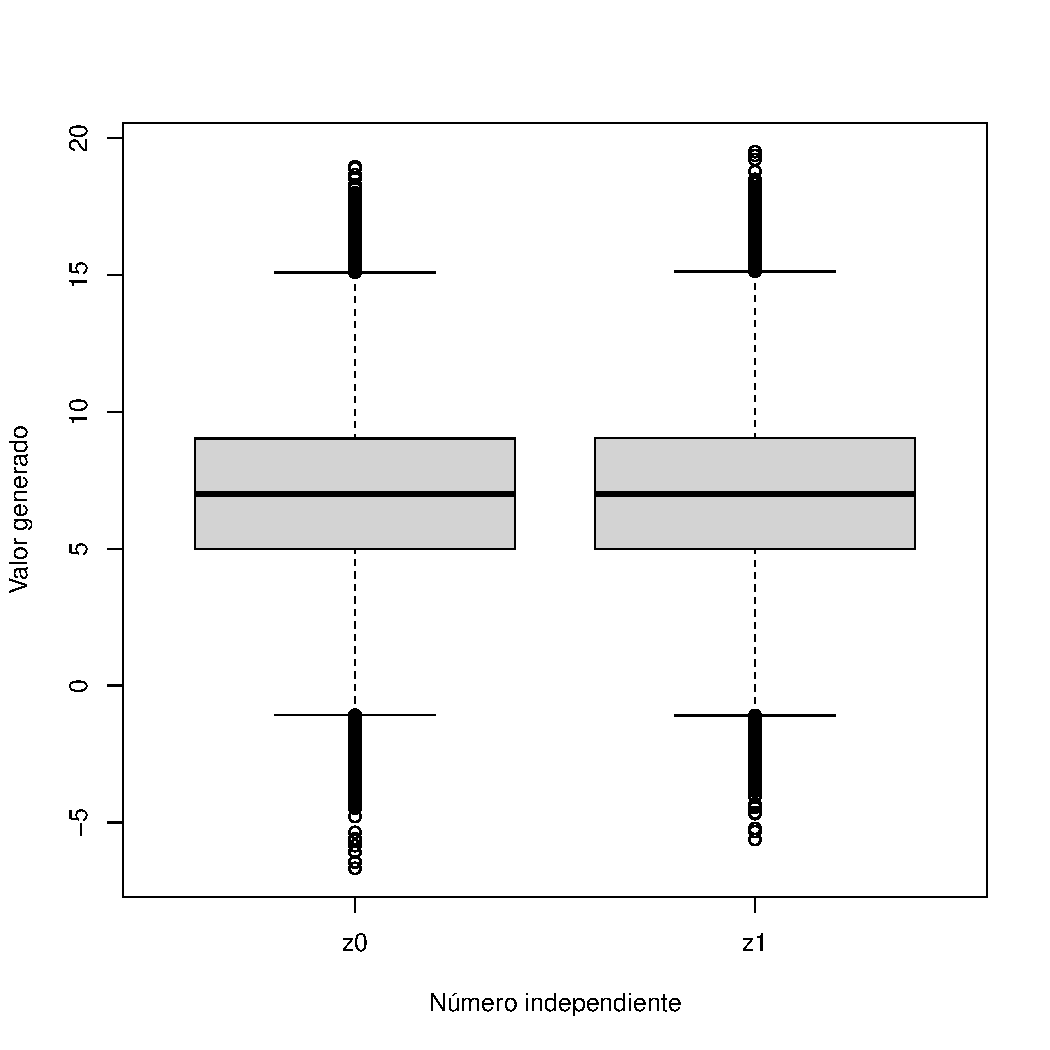
\includegraphics[width=1\textwidth]{gaussian_boxplot.pdf}
    \caption{Diagramas de cajas y bigotes de $100000$ valores generados de dos números independientes $z_0, z_1$ a partir de un algoritmo que parte del método de Box--Muller.}
    \label{gaussian_boxplot}
\end{figure}

\subsection{Cambios en distribuciones de $u_1$ y $u_2$}
Se probará ahora utilizar otras distribuciones de las que partan los valores de $u_1$ y $u_2$. Se prueban las distribuciones normal, binomial y Poisson, normalizando posteriormente los valores obtenidos de cada distribución entre $[0, 1]$. Se comparan entre sí los diagramas de cajas y bigotes de estos resultados utilizando sólo los generados a partir de las $z_0$s de cada distribución, lo cual puede revisarse en la figura \ref{distribuciones} (p. \pageref{distribuciones}).

\begin{figure}
    \centering
    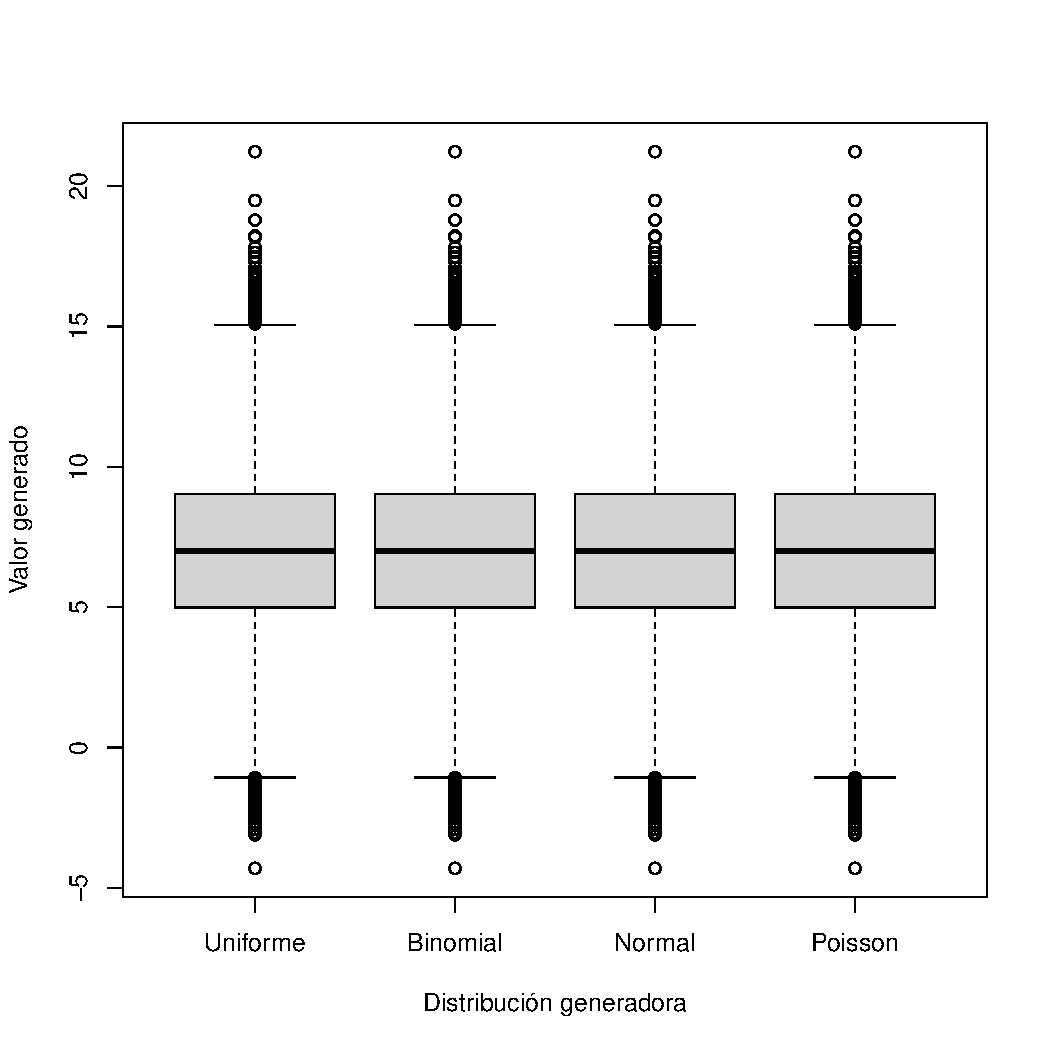
\includegraphics[width=1\textwidth]{distribuciones.pdf}
    \caption{Diagramas de cajas y bigotes de $10000$ valores generados de un números independientes $z_0$ a partir de un algoritmo que parte del método de Box--Muller con $u_1, u_2$ generados a partir de distintas distribuciones.}
    \label{distribuciones}
\end{figure}

\subsection{Valores dependientes para $u_1$ y $u_2$}
Por último, se explora cómo se comportan los números generados cuando $u_2$ depende de $u_1$. Se exploran las siguientes dependencias:
\begin{enumerate}
    \item $u_2 = 1 - u_1$,
    \item $u_2 = u_1 / 2$,
    \item $u_2 = 0.1 u_1$,
    \item $u_2 = 0.9 u_1$.
\end{enumerate}

Los resultados para cada $z_0, z_1$ de estas dependencias se muestran en la figura \ref{dependientes} (\pageref{dependientes}). Como puede constatarse, cuando los valores de $u_1$ y $u_2$ son dependientes, los números generados $z_0, z_1$ tienen distribuciones distintas que varían según la dependencia entre las variables.

\begin{figure}
    \centering
    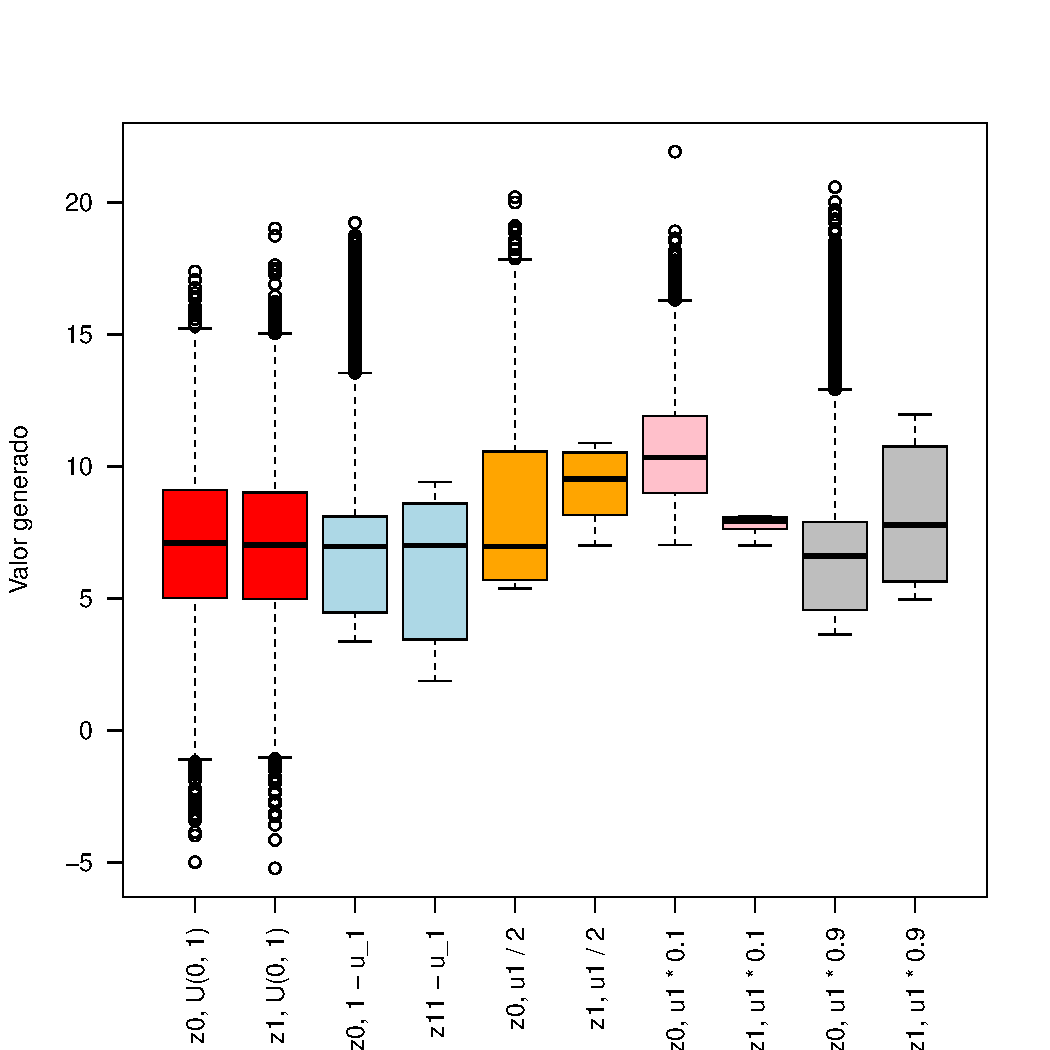
\includegraphics[width=1\textwidth]{dependientes.pdf}
    \caption{Diagramas de cajas y bigotes de $10000$ valores generados de un números independientes $z_0, z_1$ a partir de un algoritmo que parte del método de Box--Muller con $u_2$ generado a partir de $u_1$.}
    \label{dependientes}
\end{figure}

\section{Conclusiones}
Mientras los valores generadores $u_1, u_2$ sean independientes, los números pseudoaleatorios generados a partir de $z_0, z_1$ mantienen distribuciones similares, contrario a lo que sucede cuando $u_1, u_2$ no son independientes entre sí. 

\bibliographystyle{plainnat}
\bibliography{Biblio}

\end{document}